\documentclass[12pt, a4paper, twoside]{article}
\usepackage[margin=1in, headheight=0.3in, headsep=0.2in]{geometry}
\textwidth 16.5 cm \textheight 24cm
\oddsidemargin -2mm

% Packages
\usepackage{amsmath, listings, xcolor, tcolorbox, microtype, fancyhdr, hyperref, tikz, float, physics}
\usetikzlibrary{decorations.pathreplacing}

% Configure text justification
\raggedbottom
\renewcommand{\textfraction}{0.05}
\renewcommand{\floatpagefraction}{0.85}
\renewcommand{\topfraction}{0.9}

% Configure the header
\setlength{\headheight}{14.49998pt}
\pagestyle{fancy}
\fancyhf{} 
\fancyhead[L]{\leftmark}
\fancyhead[R]{\thepage}
\renewcommand{\footrulewidth}{0pt}
\renewcommand{\sectionmark}[1]{\markboth{\thesection.~#1}{}}
\renewcommand{\subsectionmark}[1]{}

% Configure the links to look professional
\hypersetup{
    colorlinks=true,      % false: boxed links; true: colored links
    linkcolor=navyblue,   % Color of internal links (TOC, sections)
    citecolor=navyblue,   % Color of citations
    urlcolor=navyblue,    % Color of external URLs
    pdftitle={Numerical Solutions using WKB},  % Metadata for the PDF
    pdfauthor={Mohak Das}                      % Metadata for the PDF
}

% Define custom colors for code
\definecolor{codegreen}{rgb}{0,0.6,0}
\definecolor{codegray}{rgb}{0.2,0.2,0.2}
\definecolor{codepurple}{rgb}{0.58,0,0.82}
\definecolor{backcolour}{rgb}{0.95,0.95,0.92}
\definecolor{navyblue}{RGB}{0, 51, 102} % A professional deep blue

% Configure the Fortran style
\lstdefinestyle{codestyle}{
    backgroundcolor=\color{backcolour},   
    commentstyle=\color{codegreen},
    keywordstyle=\color{magenta},
    numberstyle=\tiny\color{codegray},
    stringstyle=\color{codepurple},
    basicstyle=\ttfamily\footnotesize, % Typewriter font, small size
    breakatwhitespace=false,         
    breaklines=true,                 % Break long lines automatically
    captionpos=b,                    % Caption at bottom
    keepspaces=true,                 
    numbers=left,                    % Line numbers on the left
    numbersep=5pt,                  
    showspaces=false,                
    showstringspaces=false,
    showtabs=false,                  
    tabsize=4,
    language=Fortran                 % Set language to Fortran
}

% Define a style for raw text output
\lstdefinestyle{outputstyle}{
    backgroundcolor=\color{white},   
    basicstyle=\ttfamily\small,      % Monospaced font
    breaklines=true,                 % Wrap long lines
    frame=single,                    % Add a black frame around the output
    numbers=none,                    % No line numbers
    captionpos=b,
    keepspaces=true
}

\begin{document}

    \begin{titlepage}
        \centering

        \vspace*{\fill}
        \Huge \textsc{\textcolor{navyblue}{Jadavpur University}}\\
        \LARGE \textsc{Department of Physics}\\[1cm]

        \textcolor{navyblue}{\rule{\linewidth}{0.8mm}} \\[0.4cm] 
        \Huge \textbf{\textcolor{navyblue}{Numerical Integration using the \\ Monte Carlo Simulation}} \\[0.2cm]
        \textcolor{navyblue}{\rule{\linewidth}{0.8mm}} \\[1.5cm] 

        \large \textit{Monte Carlo Integration}\\[0.5cm]

        \begin{tcolorbox}[colback=navyblue!5!white, colframe=navyblue, width=0.8\textwidth, boxrule=0.5mm, arc=2mm, auto outer arc]
            \centering \Large
            $$ \int_{a}^{b} f(x) \, dx ~\approx~ (b-a)\frac{1}{N}\sum_{i=1}^{N}f(x_i)$$
        \end{tcolorbox}

        \vspace{1.5cm}

        \noindent
        \begin{minipage}{0.4\textwidth}
            \begin{flushleft} \Large
                \textbf{Submitted by:}\\
                \textcolor{navyblue}{Mohak Das}\\
            \end{flushleft}
        \end{minipage}
        \begin{minipage}{0.4\textwidth}
            \begin{flushright} \Large
                \textbf{Supervisor:} \\
                Dr. Sahinur Reja\\
                \vspace{0.6cm}
            \end{flushright}
        \end{minipage}
        \vspace{1cm}

        \textbf{Class:} PG-I\\
        \textbf{Class Roll No:} 002520702028\\
        \textbf{Exam Roll No:} PPHD0261034
        \vspace{1.5cm}

        \textsc{Computational Physics Lab}

        \vspace*{\fill}


    \end{titlepage}
    \thispagestyle{empty}

    \begin{abstract}
        This report investigates the application and statistical validity of Monte Carlo computational methods for solving deterministic integration problems. By utilizing pseudorandom number generation, both the Hit-or-Miss (rejection) method and the Mean Value (sample average) method are implemented to evaluate integrals across single and multiple dimensions. The study spans fundamental geometric estimations, such as the computation of $\pi$, to complex multi-dimensional surface volumes bounded by non-linear constraints, including a paraboloid over a circular domain. A central focus is placed on the rigorous empirical verification of the algorithm's statistical error. Through logarithmic curve fitting of the absolute error against the number of iterations ($N$), the results successfully demonstrate that the integration error strictly adheres to the $O(N^{-0.5})$ convergence rate dictated by the Central Limit Theorem, completely independent of the integral's dimensionality.
    \end{abstract}
    
    \thispagestyle{empty}
    \newpage

  	\tableofcontents
	\thispagestyle{empty}
	
	\clearpage
	\pagenumbering{arabic}

    \section{Introduction}

       Numerical integration is a cornerstone of computational physics, essential for evaluating complex systems where analytical solutions are either intractable or impossible. While traditional deterministic algorithms, such as Simpson's rule or Gaussian quadrature, are highly efficient for one-dimensional problems, they suffer severely from the "curse of dimensionality." As the number of variables increases, the computational cost of grid-based methods grows exponentially. Monte Carlo methods bypass this limitation by employing statistical randomness to approximate definite integrals, offering a convergence rate that remains invariant regardless of the system's dimensions.
       
       This report explores two distinct Monte Carlo architectures:
       \begin{enumerate}
        \item {\bf The Hit-or-Miss Method:} A geometric approach that frames integration as a probability problem. By enclosing a target region within a known bounding volume and generating uniform random coordinates, the integral is estimated by the ratio of "accepted" points that satisfy the bounding condition to the total number of samples.
        \item  {\bf The Mean Value Method:} A statistical approach derived from the Mean Value Theorem for Definite Integrals. It approximates the integral by uniformly sampling the domain and calculating the expected (average) value of the function, scaled by the total volume of the integration space.
       \end{enumerate}
       
      A defining characteristic of all Monte Carlo integration is its reliance on the Law of Large Numbers and the Central Limit Theorem. Unlike deterministic methods, the error in a Monte Carlo simulation is inherently statistical. Theory dictates that the standard deviation of the estimate and thus the absolute error decreases proportionally to $\frac{1}{\sqrt{N}}$, where $N$ is the number of random samples.In this study, these theoretical frameworks are translated into highly optimized, vectorized computational algorithms. By evaluating a series of progressively complex geometries ranging from one-dimensional trigonometric functions to bounded three-dimensional surfaces, this report systematically visualizes the sampling behavior, tests the computational accuracy against exact analytical solutions, and rigorously proves the universal $N^{-0.5}$ error convergence rate.

    \section{Numerical Implementation}

        \subsection{Global Constants and Precision}
        To ensure numerical stability and physical consistency across all problems, a shared module \texttt{constants\_mod} is used. This module defines the double-precision floating-point kind (\texttt{real64}).

        \lstinputlisting[caption={Global Constants Module}, style= codestyle, label={lst:const}]{src/shared/constants_mod.f90}

        \subsection{The General Monte Carlo Solver}
        The core logic is encapsulated in the \texttt{monte\_carlo\_toolbox} module.
        This module consist of various functionality that is directly or indirectly solving the assignment problems. Here is the explanation:
        \begin{enumerate}
            \item {\bf \texttt{uniform}:} This subroutine takes generates uniformly distributed random numbers in the domain $[a, b)$. It uses \texttt{random\_number} subroutine which generates uniformly distributed random numbers between $0$ and $1$ and by mathematical transformation $x = a + (b - a)r$ it scales the existing random numbers $(r)$ in our desired domain $[a, b)$.
            \item {\bf \texttt{MCI\_1D}:} This function finds area made with $x$ axis by a single curve using Monte Carlo mean-value method. It takes the integrand, lower bound, upper bound, number of random points and returns the area under the curve.
            \item {\bf \texttt{MCI\_2D}:} This function finds volume made with $xy$ plane by a surface (2D integrand) using Monte Carlo mean-value method. It takes the integrand, lower bound, upper bound (for both $x$ and $y$ axis), number of random points and returns the volume under the surface.
            \item {\bf \texttt{MC\_area\_single}:} This function finds area made with $x$ axis by a single curve using Monte Carlo sampling method. It takes integrand, lower bound, upper bound, number of random points and returns the area under the curve.
            \item {\bf \texttt{MC\_area\_dual}:} This function finds area between two curve using Monte Carlo sampling method. It takes integrands, lower bound, upper bound, number of random points and returns the area between the curve.
            \item {\bf \texttt{MC\_volume\_2D}:} This function finds volume made with $xy$ plane by a surface (2D integrand) using Monte Carlo sampling method. It takes integrand, lower bound, upper bound, number of random points, the boundary of points counting and returns the volume under the surface.
        \end{enumerate}
        \lstinputlisting[caption={MC Toolbox Implementation}, style= codestyle, label={lst:solver}]{src/shared/monte_carlo_toolbox.f90}
        
        \section{Area Under a Curve Using Monte Carlo Simulation}
        \subsection{Problem 1: Area Under a Polynomial Curve}
        \begin{itemize}
            \item {\bf Function: } $f(x) = x^2$ in the interval $0 \leq x \leq 1$.
            \item {\bf Code: } Monte carlo hit-or-miss method is used.\lstinputlisting[style= codestyle]{src/problems/prob01_area_under_curve.f90}
            \item {\bf Sampling Plot: } The function $f(x) = x^2$ is plotted along with the randomly generated points inside the $1 \cross 1$ rectangular grid. The 'Black' points reside outside the curve and the 'Violet' points reside inside the curve traced by the function. \begin{figure}[H]
                \centering
                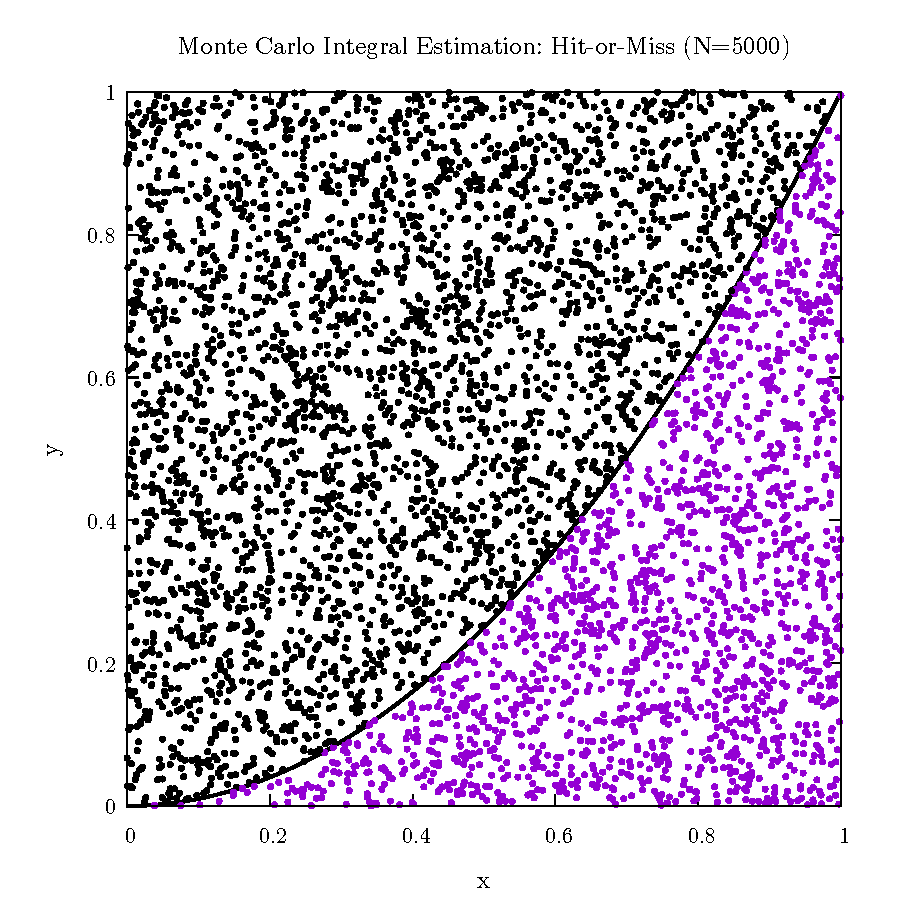
\includegraphics[width=0.6\textwidth]{plots/prob01_sampling.pdf}
                \label{fig1:prob01_sampling}
            \end{figure}
            \item {\bf Output: } Comparison with the exact value.\lstinputlisting[style= outputstyle]{output/prob01_output.txt}
            \item {\bf Convergence Plot: } \begin{figure}[H]
                \centering
                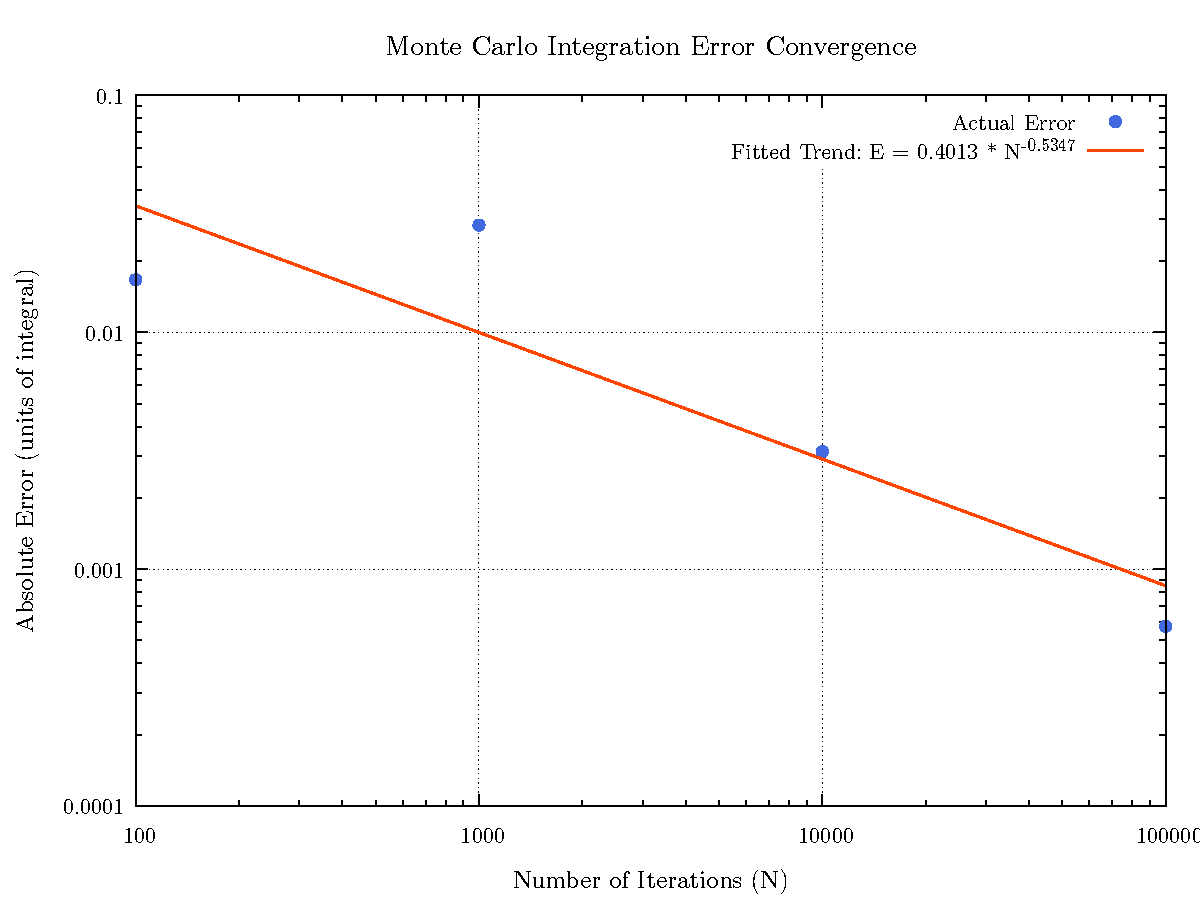
\includegraphics[width=0.6\textwidth]{plots/prob01_error.pdf}
                \label{fig2:prob01_error}
            \end{figure} The log log plot of error convergence against the number of random points $(N)$ with a slope $\approx 0.5$ successfully shows that the error propagation in Monte Carlo method is proportional to $\frac{1}{\sqrt{N}}$ where, $N$ is the number of points injected inside the rectangular grid.
        \end{itemize}
        
        \subsection{Problem 2: Area Under a Trigonometric Function}
        \begin{itemize}
            \item {\bf Function: } $f(x) = \sin{x}$ for $0 \leq x \leq \pi$. For this problem, the bounding rectangle will have length of $\pi$ unit $(0 \leq x \leq \pi)$ and breadth of 1 unit $(0 \leq y \leq 1)$ as $\sin{x}$ has upper bound of 1.
            \item {\bf Code: } Monte Carlo sampling method is used. \lstinputlisting[style= codestyle]{src/problems/prob02_area_under_trigfunc.f90}
            \item {\bf Sampling Plot: } The function $f(x) = \sin{x}$ is plotted along with the randomly generated points inside the $\pi \cross 1$ rectangular grid. The 'Black' points reside outside the curve and the 'Violet' points reside inside the curve traced by the function. \begin{figure}[H]
                \centering
                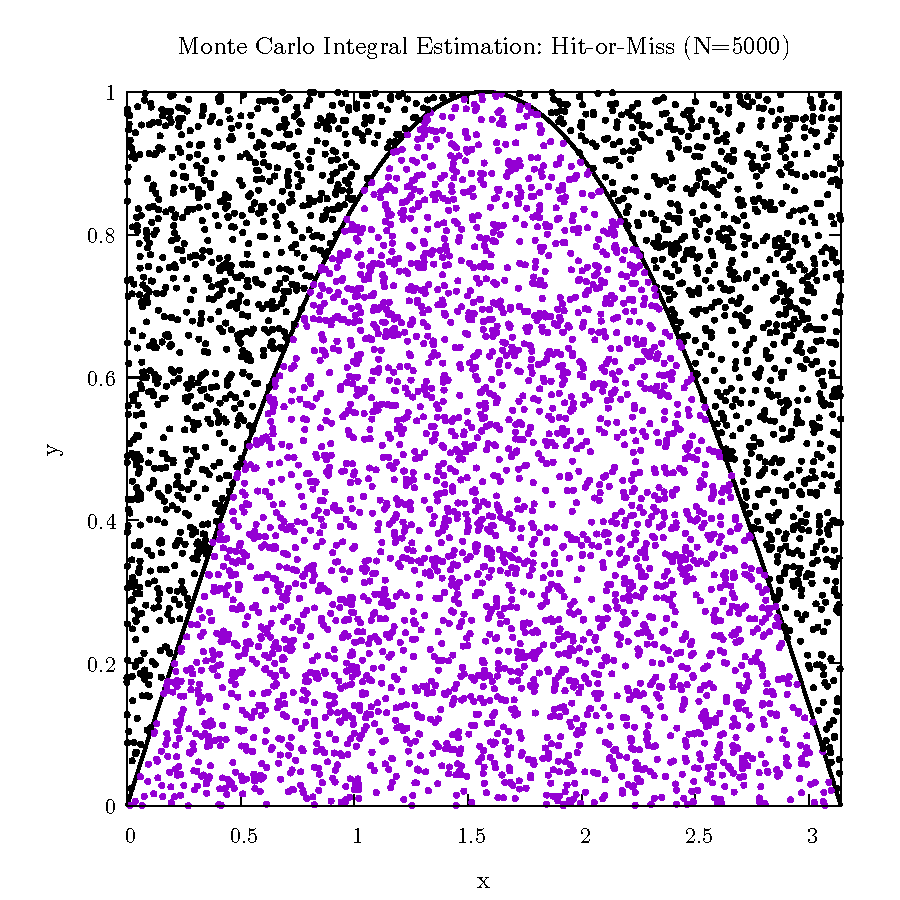
\includegraphics[width=0.6\textwidth]{plots/prob02_sampling.pdf}
                \label{fig3:prob02_sampling}
            \end{figure}
            \item {\bf Output: } \lstinputlisting[style= outputstyle]{output/prob02_output.txt}
            \item {\bf Convergence Plot: } \begin{figure}[H]
                \centering
                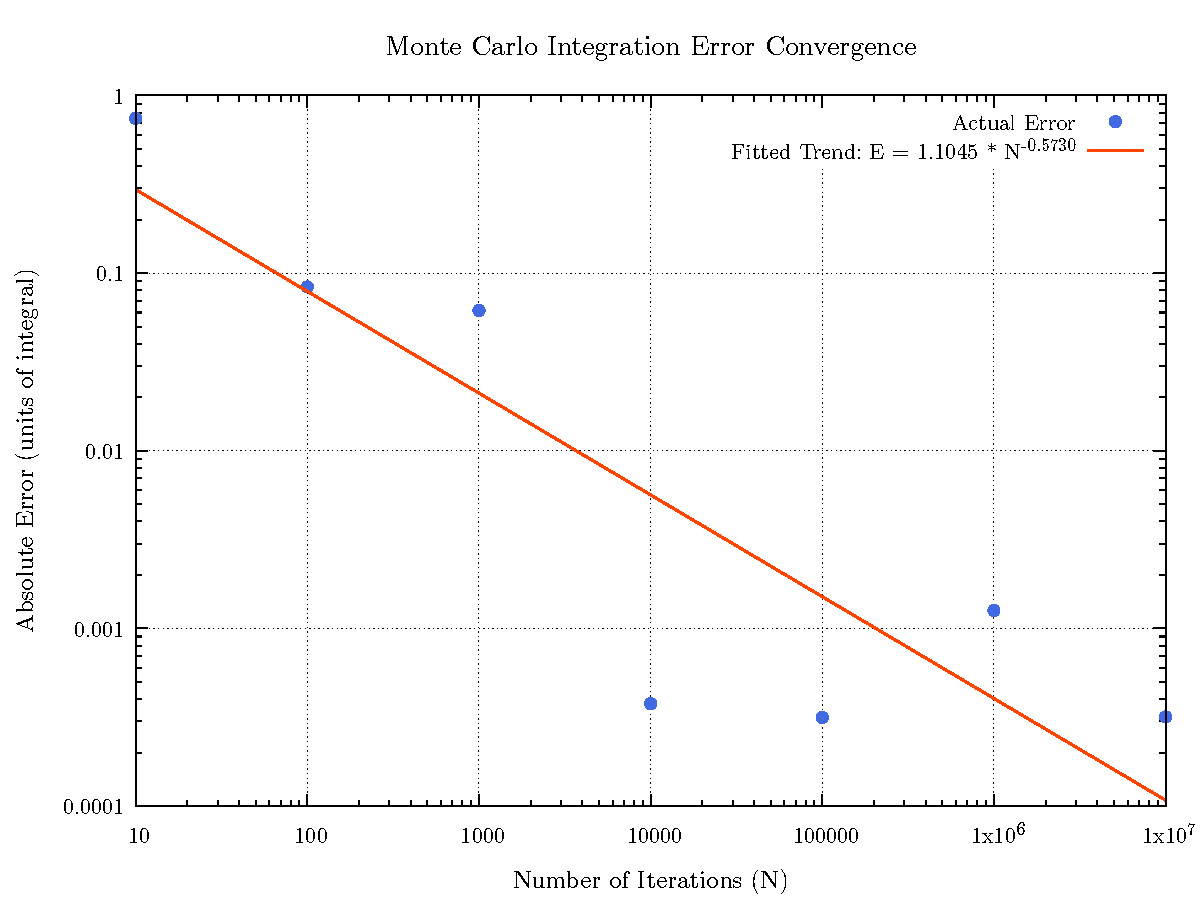
\includegraphics[width=0.6\textwidth]{plots/prob02_error.pdf}
                \label{fig4:prob02_error}
            \end{figure} The log log plot of error convergence against the number of random points $(N)$ with a slope $\approx 0.5$ successfully shows that the error propagation in Monte Carlo method is proportional to $\frac{1}{\sqrt{N}}$ where, $N$ is the number of points injected inside the rectangular grid.
        \end{itemize}
        
        \subsection{Problem 3: Area Between Two Curves}
        \begin{itemize}
            \item {\bf Functions: } $y_1 = x^2$ and $y_2 = x$ for $0 \leq x \leq 1$. For this problem, the bounding rectangle will be a square of length of 1 unit $(0 \leq x \leq 1)$ and breadth of 1 unit $(0 \leq y \leq 1)$ as both the functions intersects at $(1, 1)$.
            \item {\bf Code: } \lstinputlisting[style= codestyle]{src/problems/prob03_area_btw_curves.f90}
            \item {\bf Sampling Plot: } The functions $y_1 = x^2$ and $y_2 = x$ are plotted along with the randomly generated points inside the $1 \cross 1$ rectangular grid. The 'Black' points reside outside the bounded region and the 'Violet' points reside inside the bounded region traced by the functions. \begin{figure}[H]
                \centering
                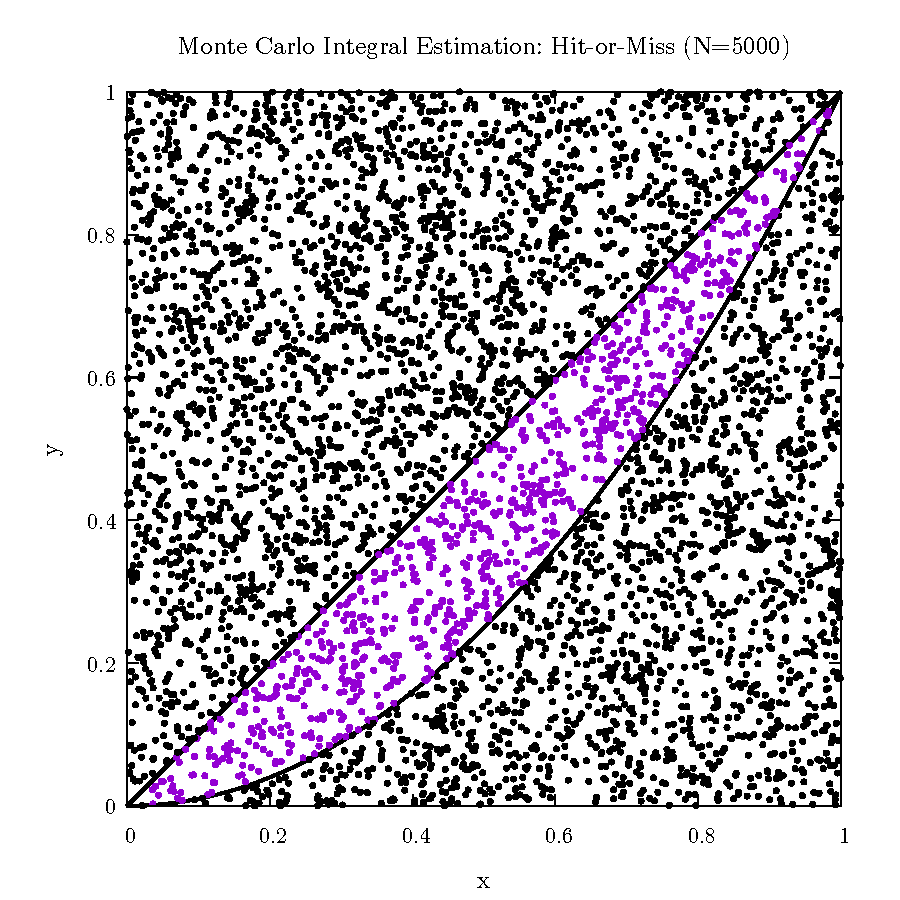
\includegraphics[width=0.6\textwidth]{plots/prob03_sampling.pdf}
                \label{fig5:prob03_sampling}
            \end{figure}
            \item {\bf Output: } \lstinputlisting[style= outputstyle]{output/prob03_output.txt}
        \end{itemize}
        
        \subsection{Problem 4: Area of a Quarter Circle}
        \begin{itemize}
            \item {\bf Function: } $y = \sqrt{1-x^2}$ for $0 \leq x \leq 1$.
            \item {\bf Code: } \lstinputlisting[style= codestyle]{src/problems/prob04_area_quarter_circle.f90}
            \item {\bf Sampling Plot: } The function $y = \sqrt{1-x^2}$ is plotted along with the randomly generated points inside the $1 \cross 1$ rectangular grid. The 'Black' points reside outside the curve and the 'Violet' points reside inside the curve traced by the quarter circle. \begin{figure}[H]
                \centering
                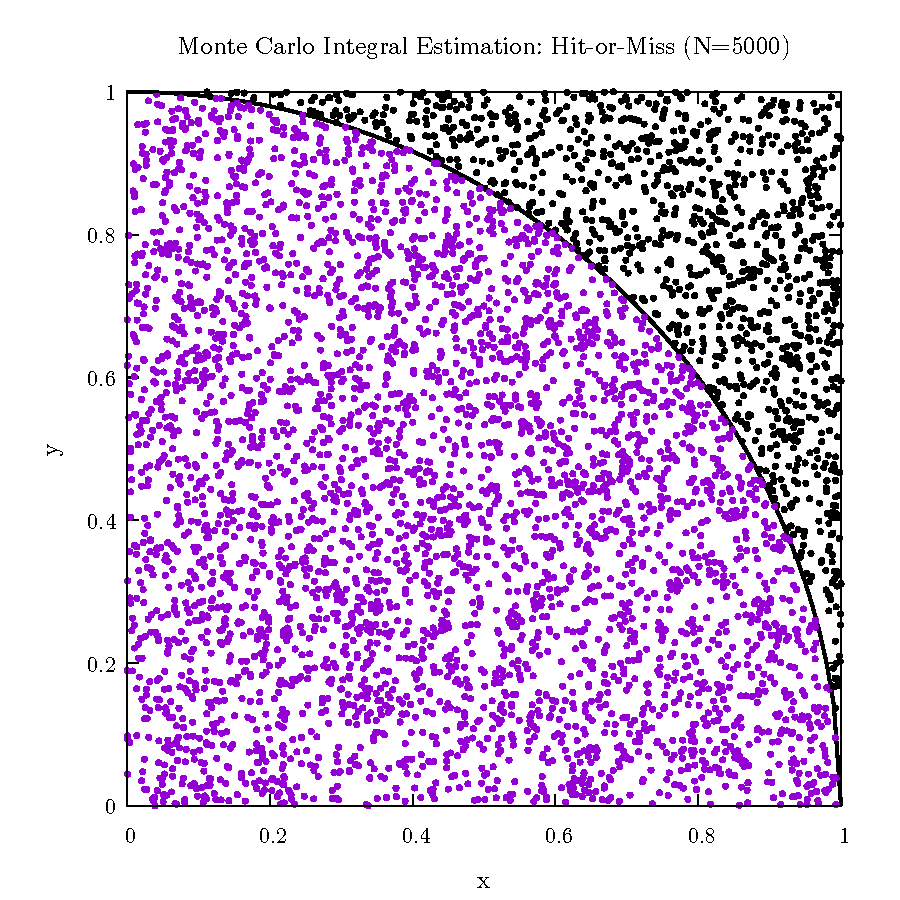
\includegraphics[width=0.6\textwidth]{plots/prob04_sampling.pdf}
                \label{fig6:prob04_sampling}
            \end{figure}
            \item {\bf Output: } \lstinputlisting[style= outputstyle]{output/prob04_output.txt}
        \end{itemize}
        
        \subsection{Problem 5: Monte Carlo Integration of a Difficult Function}
        \begin{itemize}
            \item {\bf Function: } $y = e^{-x^2}$ for $0 \leq x \leq 2$.
            \item {\bf Code: } Monte Carlo mean-value method is used. The key formula is $$A_{MC} = (b-a)\frac{1}{N}\sum_{i=1}^{N}f(x_i)$$ where $x_i$ are the uniform random numbers inside the desired integration domain. \lstinputlisting[style=codestyle]{src/problems/prob05_area_gaussian.f90}
            \item {\bf Output: } \lstinputlisting[style= outputstyle]{output/prob05_output.txt}
            \item {\bf Sampling Plot: } The functional value is calculated for the randomly generated points $x_i$ and plotted along with the function $y = e^{-x^2}$ inside the $2 \cross 1$ rectangular grid. We expect the points will be on the curve with a random distribution. \begin{figure}[H]
                \centering
                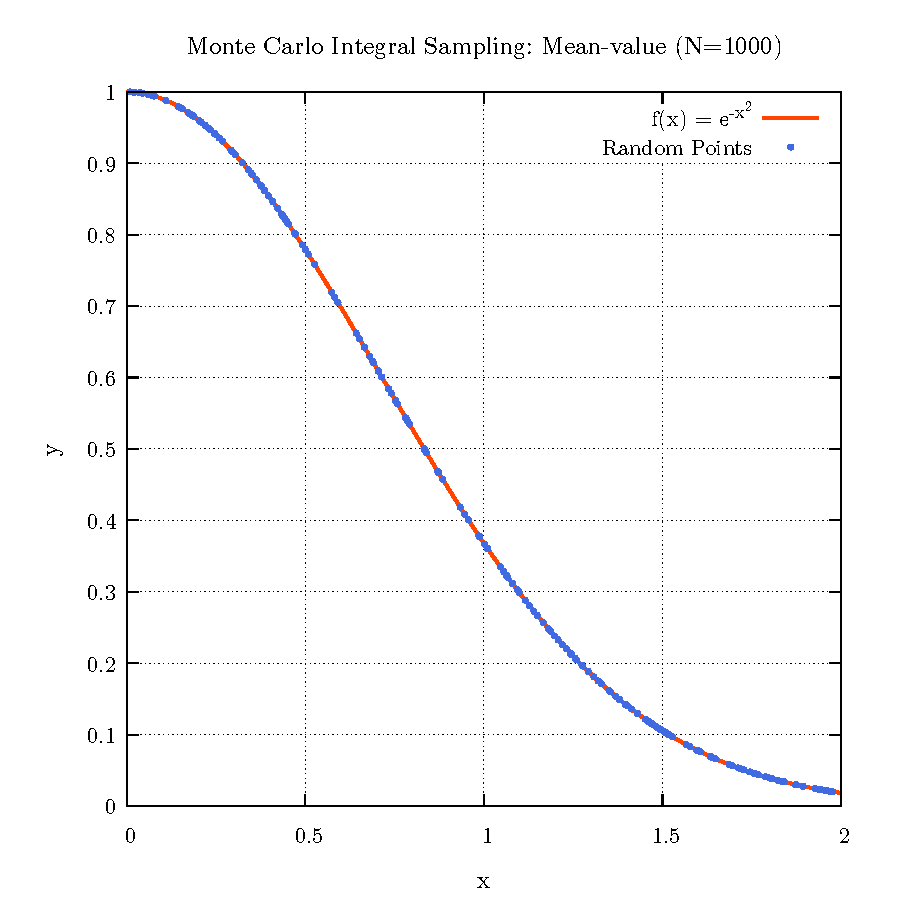
\includegraphics[width=0.6\textwidth]{plots/prob05_sampling.pdf}
                \label{fig7:prob05_sampling}
            \end{figure}
            \item {\bf Convergence Plot: } The log plot of value convergence shows that as we increase the number of random points $(N)$, the value of the integral is converging towards a specific value. For the finite interval $[0,2]$, the value is close to the infinite limit but not exactly equal. The exact value is $\frac{\sqrt{\pi}}{2} \text{erf}(2)$.\begin{figure}[H]
                \centering
                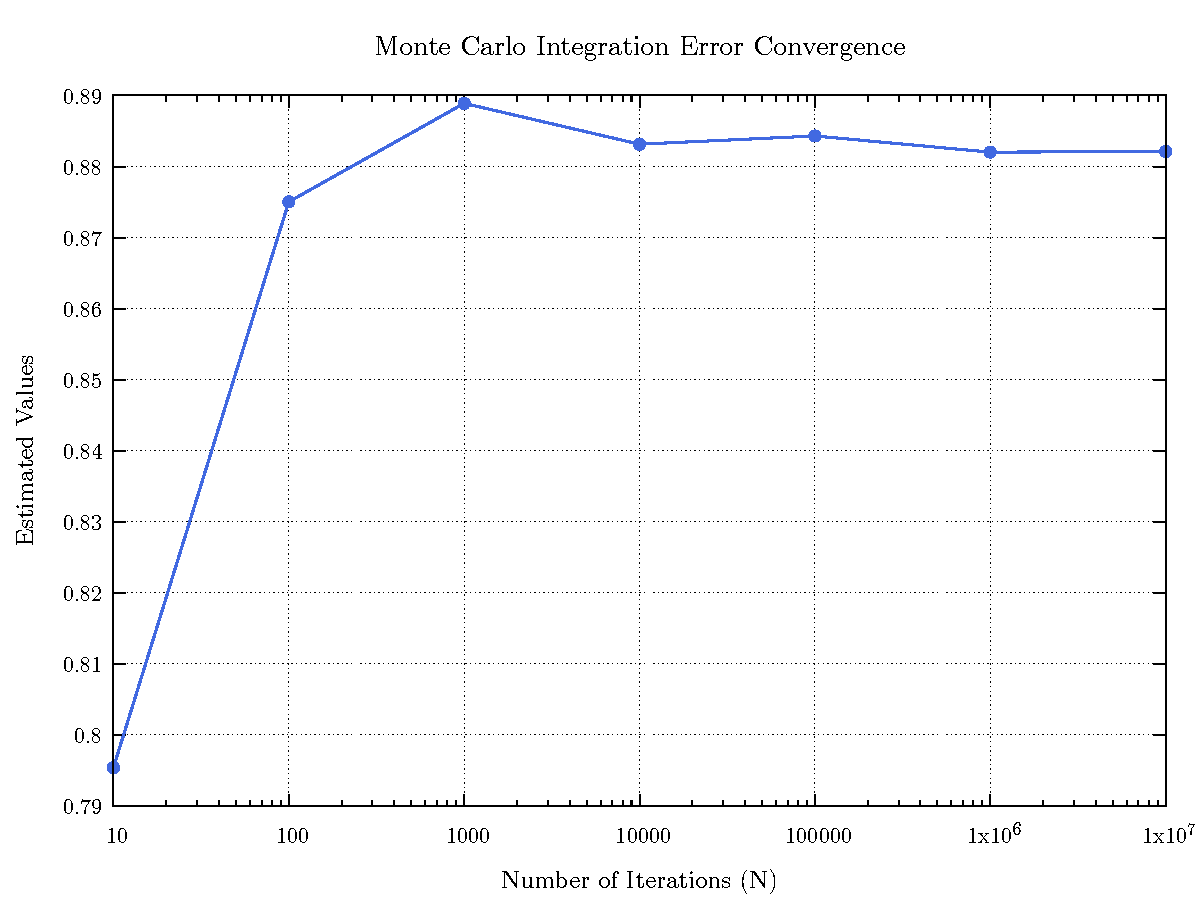
\includegraphics[width=0.6\textwidth]{plots/prob05_value_conv.pdf}
                \label{fig8:prob05_value}
            \end{figure}
        \end{itemize}
        Monte Carlo Integration is highly useful for complex, non-analytical or high-dimensional integrals because it approximates results through random sampling rather than analytical calculation. By averaging function evaluations at random points, it provides an efficient, dimension-independent convergence rate $\left(\mathcal{O}\left(\frac{1}{\sqrt{N}}\right)\right)$, making it superior for problems with high dimensions, irregular shapes, or discontinuities where traditional grid-based methods fail.
        
        \section{Monte Carlo Simulation for Area Under a Surface}
        \subsection{Problem 1: Area Under a Polynomial Curve}
        \begin{itemize}
            \item {\bf Function: } $z = x+y$ in the interval $0 \leq x \leq 1$ and $0 \leq y \leq 1$.
            \item {\bf Code: } \lstinputlisting[style= codestyle]{src/problems/prob01_area_under_curve.f90}
            \item {\bf Output: } Comparison with the exact value.\lstinputlisting[style= outputstyle]{output/prob06_output.txt}
            \item {\bf Sampling Plot: } The function $f(x, y) = x + y$ is plotted along with the randomly generated points $(x_i, y_i)$ inside the $1 \cross 1$ square grid using 3D plot. We expect the points will be on the plotted surface with a random distribution. \begin{figure}[H]
                \centering
                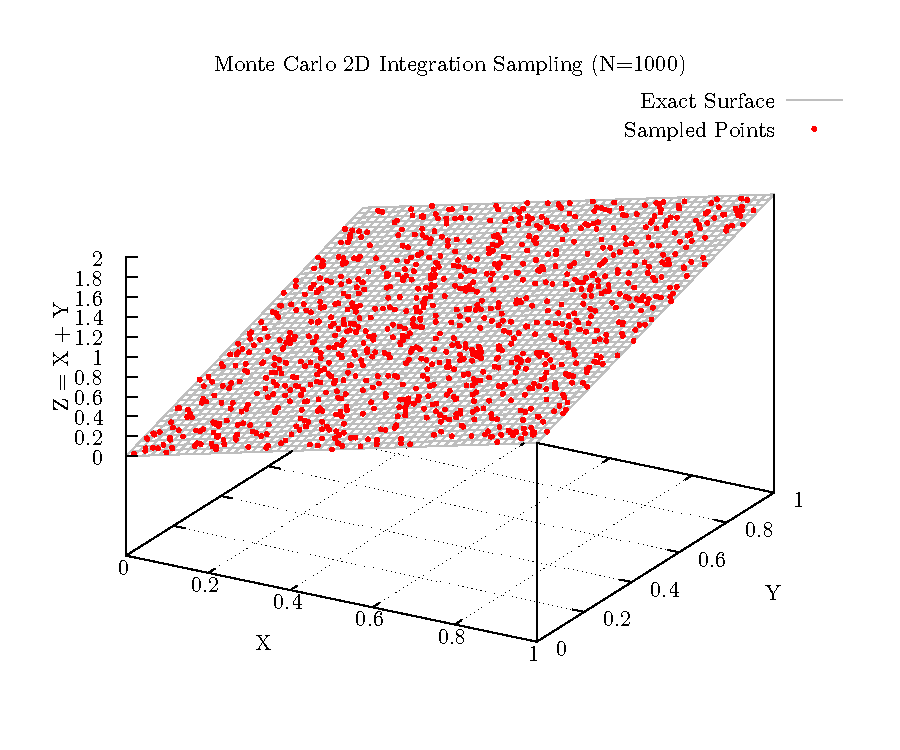
\includegraphics[width=0.6\textwidth]{plots/prob06_sampling.pdf}
                \label{fig9:prob06_sampling}
            \end{figure}
            \item {\bf Convergence Plot: } The log plot of value convergence shows that as we increase the number of random points $(N)$, the value of the integral is converging towards the analytical value "$1$". \begin{figure}[H]
                \centering
                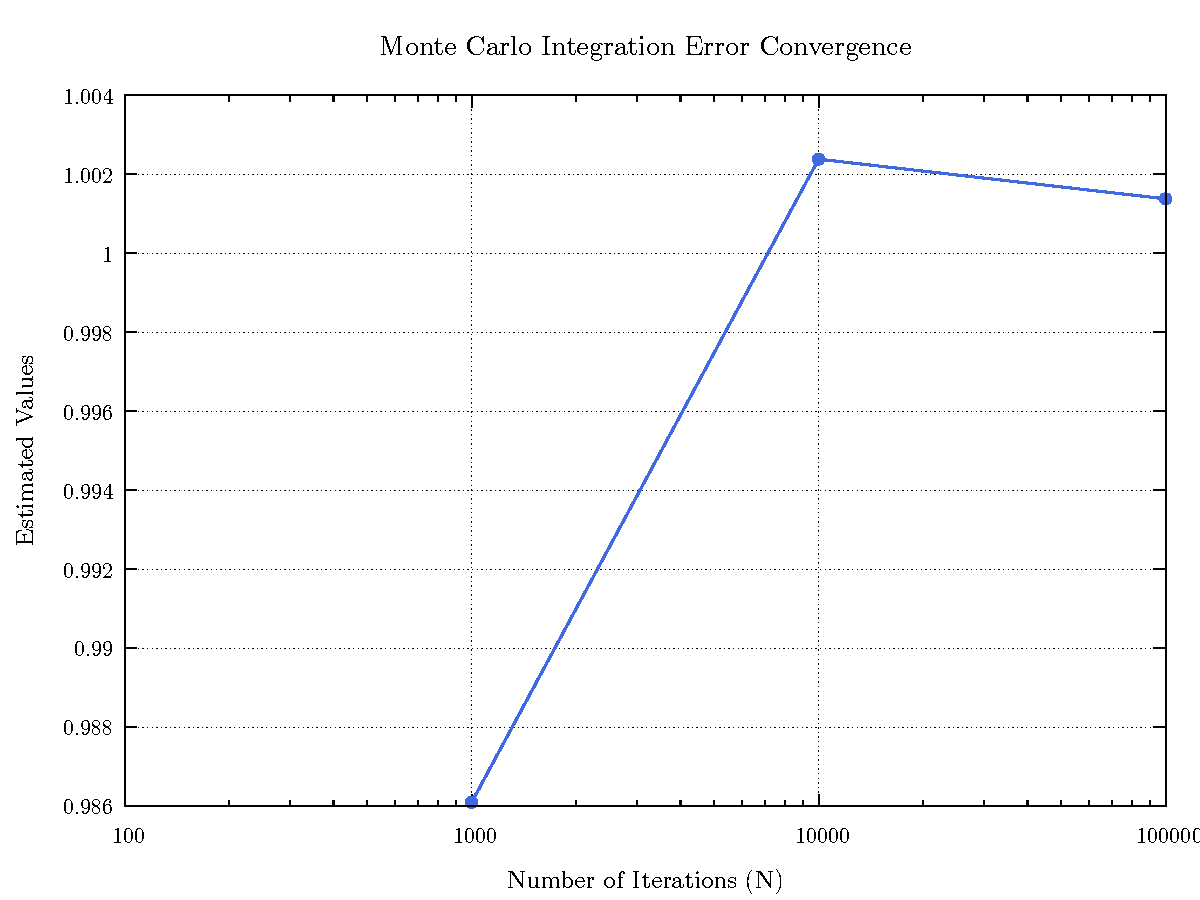
\includegraphics[width=0.6\textwidth]{plots/prob06_value_conv.pdf}
                \label{fig10:prob06_value}
            \end{figure}
        \end{itemize}
        
        \subsection{Problem 2: Parabolic Surface}
        \begin{itemize}
            \item {\bf Function: } $z = x^2 + y^2$ in the interval $0 \leq x \leq 1$ and $0 \leq y \leq 1$.
            \item {\bf Code: } \lstinputlisting[style= codestyle]{src/problems/prob07_volume_paraboloid.f90}
            \item {\bf Sampling Plot: } The function $f(x, y) = x^2 + y^2$ is plotted along with the randomly generated points $(x_i, y_i)$ inside the $1 \cross 1$ square grid using 3D plot. We expect the points will be on the plotted surface with a random distribution. \begin{figure}[H]
                \centering
                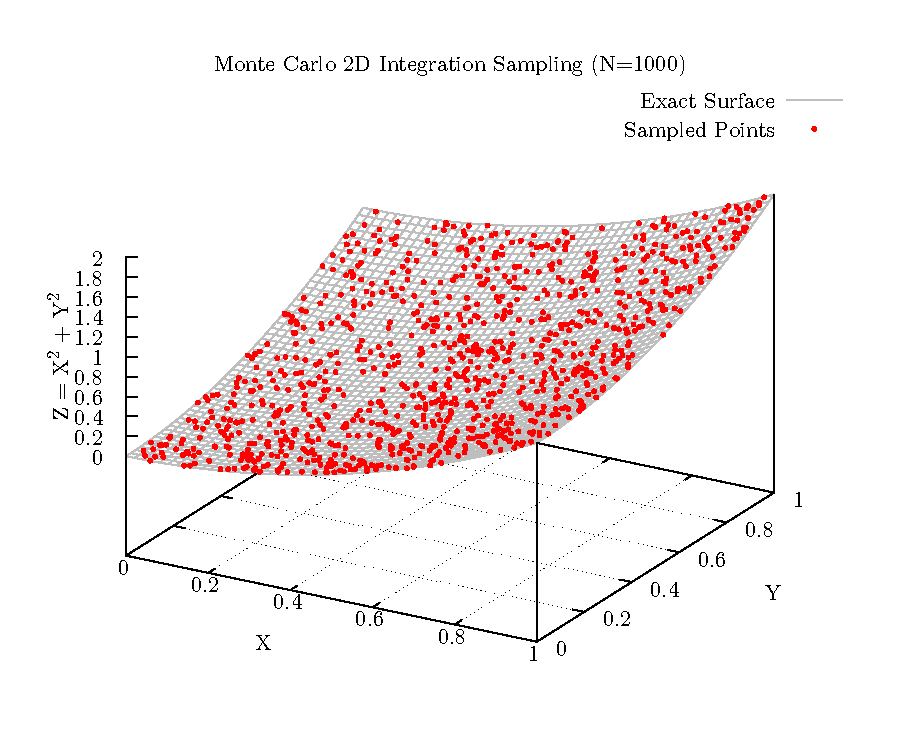
\includegraphics[width=0.6\textwidth]{plots/prob07_sampling.pdf}
                \label{fig11:prob07_sampling}
            \end{figure}
            \item {\bf Output: } Comparison with the exact value.\lstinputlisting[style= outputstyle]{output/prob07_output.txt}
            \item {\bf Convergence Plot: } \begin{figure}[H]
                \centering
                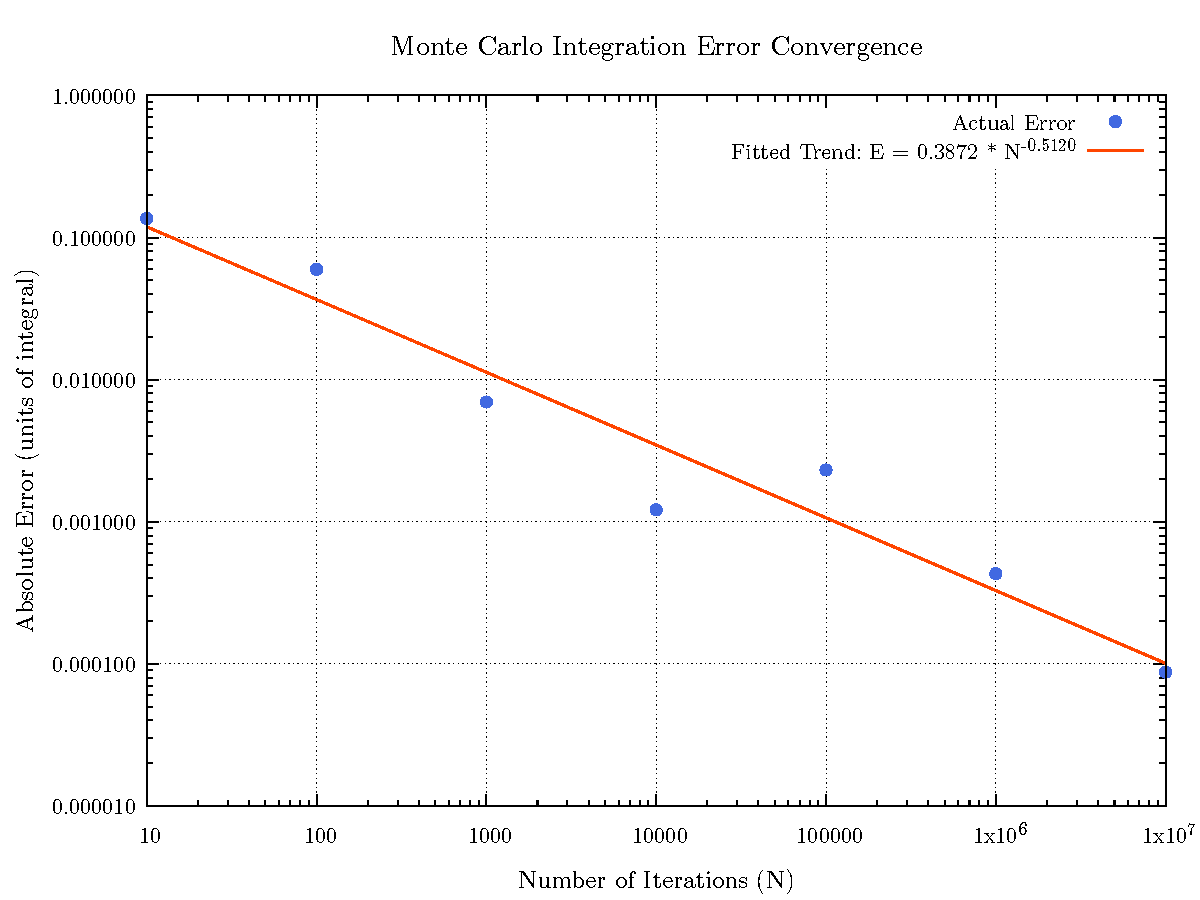
\includegraphics[width=0.6\textwidth]{plots/prob07_error.pdf}
                \label{fig12:prob07_error}
            \end{figure} The log log plot of error convergence against the number of random points $(N)$ with a slope $\approx 0.5$ successfully shows that the error propagation in Monte Carlo method is proportional to $\frac{1}{\sqrt{N}}$ where, $N$ is the number of points injected inside the square grid.
        \end{itemize}
        
        \subsection{Problem 3: Surface Over a Circular Region}
        \begin{itemize}
            \item {\bf Function: } $z = x^2 + y^2$ in the interval $0 \leq x \leq 1$ inside the unit circle $x^2+y^2 \leq 1$.
            \item {\bf Code: } \lstinputlisting[style= codestyle]{src/problems/prob08_circular_surface.f90}
            \item {\bf Output: } \lstinputlisting[style= outputstyle]{output/prob08_output.txt}
            \item {\bf Sampling Plot: } The randomly generated points are plotted in a $1 \cross 1$ square grid. The 'Violet' points satisfies the condition $x^2 + y^2 \leq 1$ the 'Black' points violates this condition. \begin{figure}[H]
                \centering
                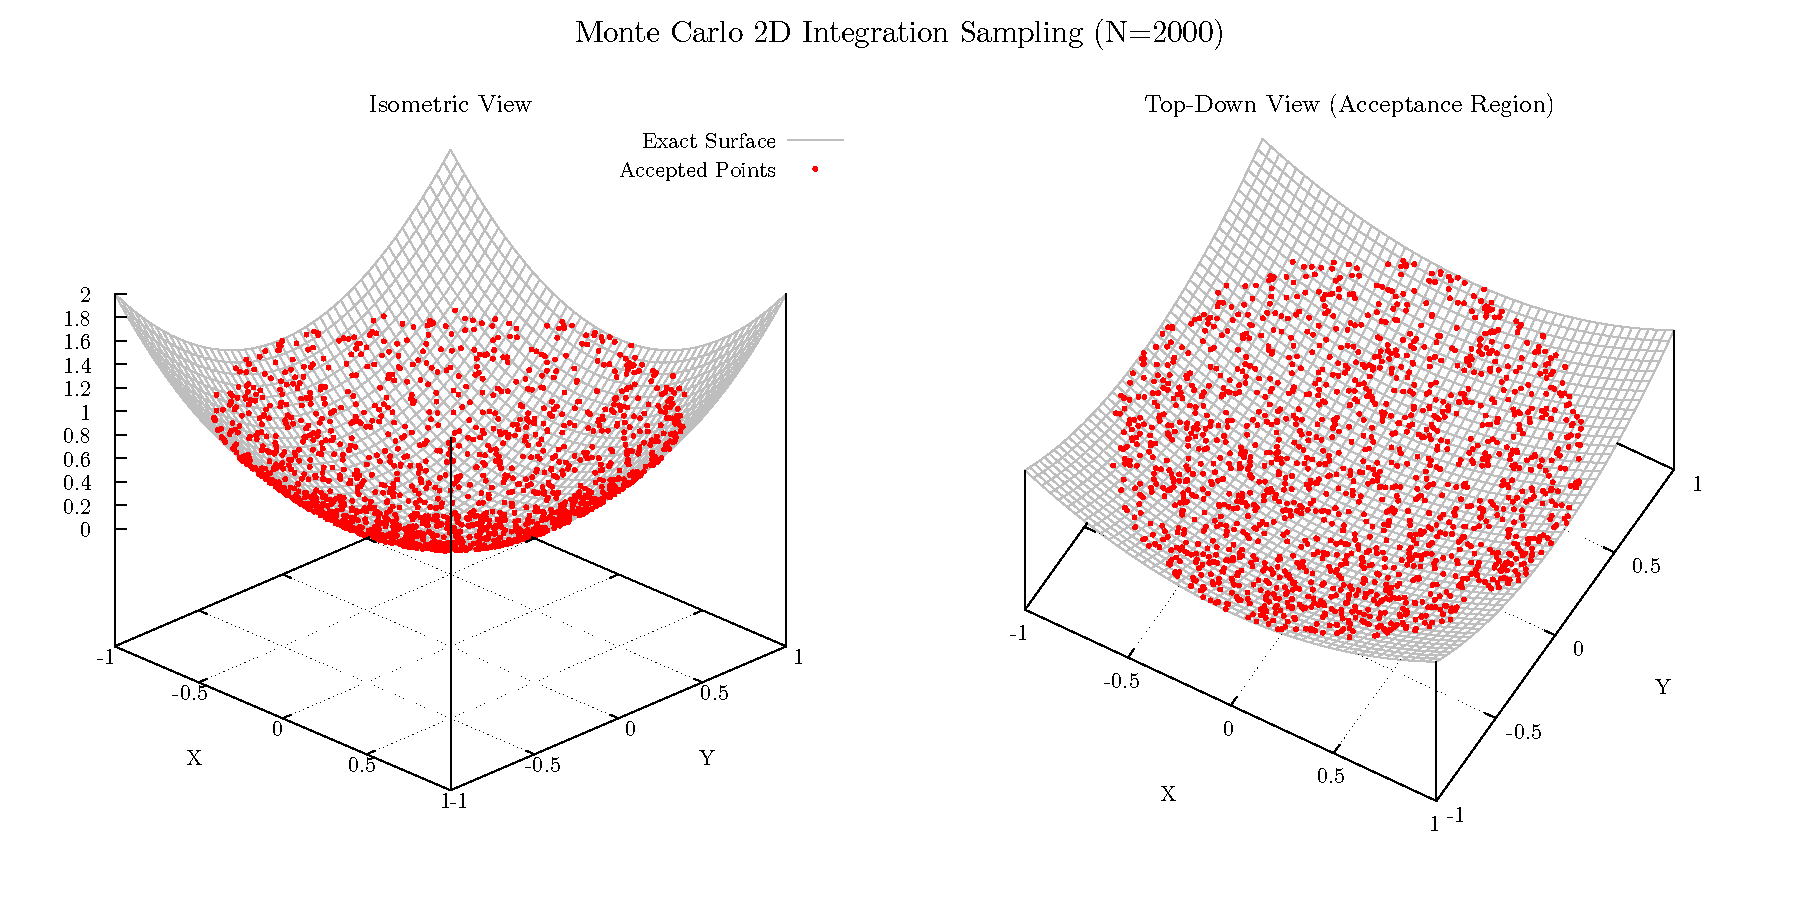
\includegraphics[width=0.8\textwidth]{plots/prob08_multiview.pdf}
                \label{fig13:prob08_sampling}
            \end{figure}
        \end{itemize}

        \subsection{Problem 4: Exponential Surface}
        \begin{itemize}
            \item {\bf Function: } $z = e^{-(x^2+y^2)}$ for $-2 \leq x \leq 2$ and $-2 \leq x \leq 2$.
            \item {\bf Code: } \lstinputlisting[style=codestyle]{src/problems/prob09_volume_gaussian.f90}
            \item {\bf Sampling Plot: } The function $f(x, y) = x^2 + y^2$ is plotted along with the randomly generated points $(x_i, y_i)$ inside the $4 \cross 4$ square grid using 3D plot. We expect the points will be on the plotted surface with a random distribution. \begin{figure}[H]
                \centering
                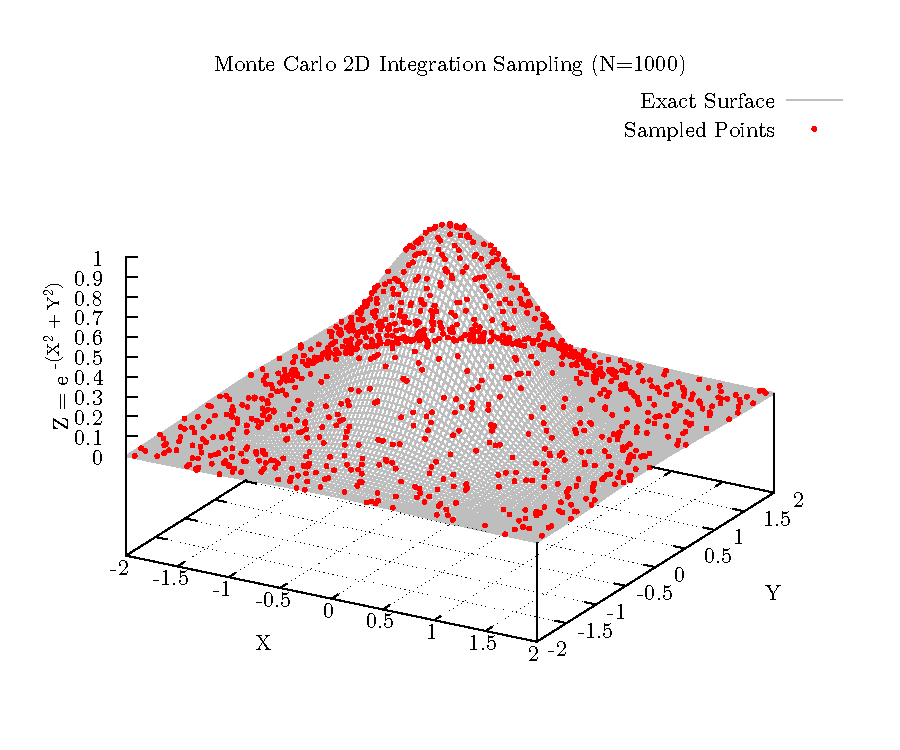
\includegraphics[width=0.6\textwidth]{plots/prob09_sampling.pdf}
                \label{fig14:prob09_sampling}
            \end{figure}
            \item {\bf Output: } \lstinputlisting[style= outputstyle]{output/prob09_output.txt}
            \item {\bf Convergence Plot: } The log plot of value convergence shows that as we increase the number of random points $(N)$, the value of the integral is converging towards a specific value (around $\pi$ solved using polar coordinates.)\begin{figure}[H]
                \centering
                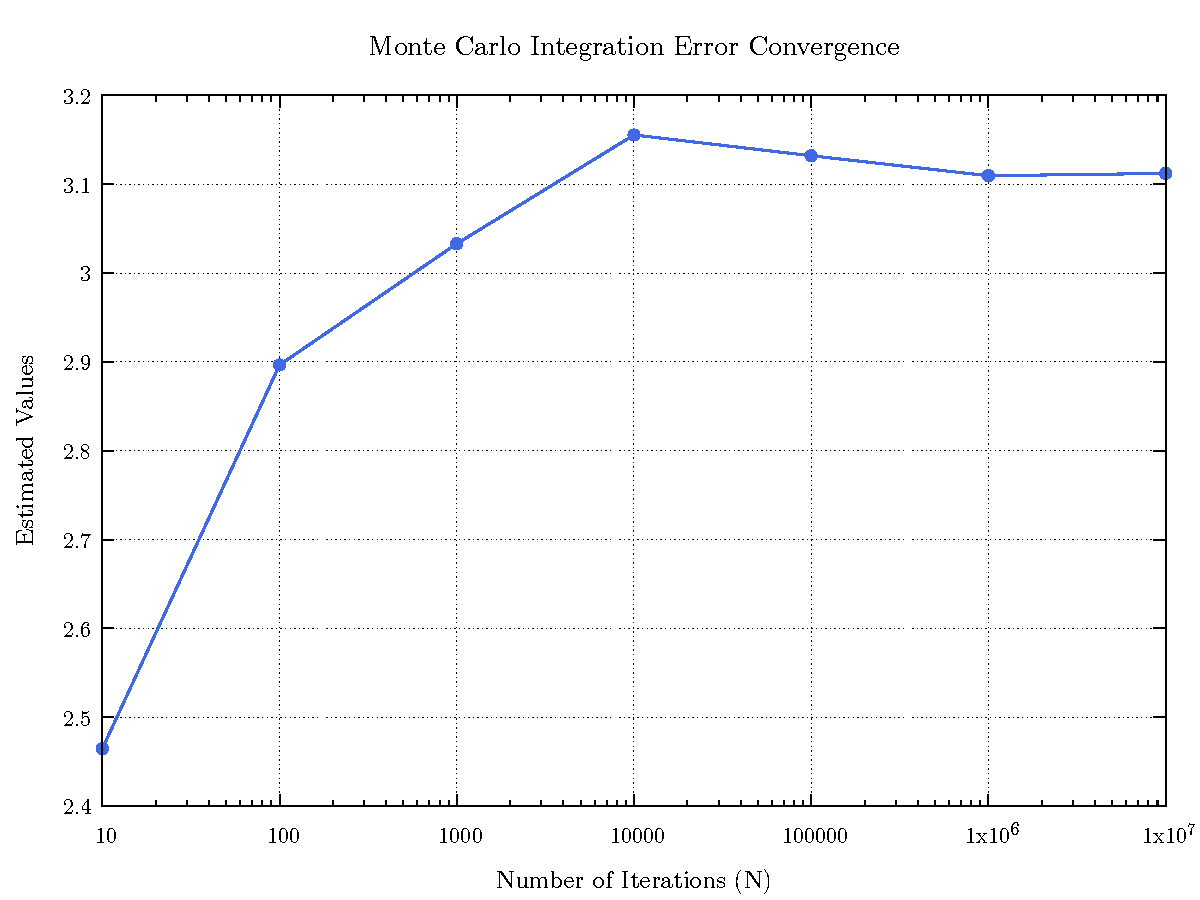
\includegraphics[width=0.6\textwidth]{plots/prob09_value_conv.pdf}
                \label{fig15:prob09_value}
            \end{figure}
        \end{itemize}

        \subsection{Problem 5: Volume Between Two Surfaces}
        \begin{itemize}
            \item {\bf Function: } $z_1 = x + y$ and $z_2 = x^2+y^2$ for $0 \leq x \leq 1$ and $0 \leq x \leq 1$.
            \item {\bf Code: } \lstinputlisting[style=codestyle]{src/problems/prob10_volume_btw_surfaces.f90}
            \item {\bf Sampling Plot: } The function $f(x, y) = (x + y) - (x^2 + y^2)$ is plotted along with the randomly generated points $(x_i, y_i)$ inside the $1 \cross 1$ square grid using 3D plot. We expect the points will be on the plotted surface with a random distribution. \begin{figure}[H]
                \centering
                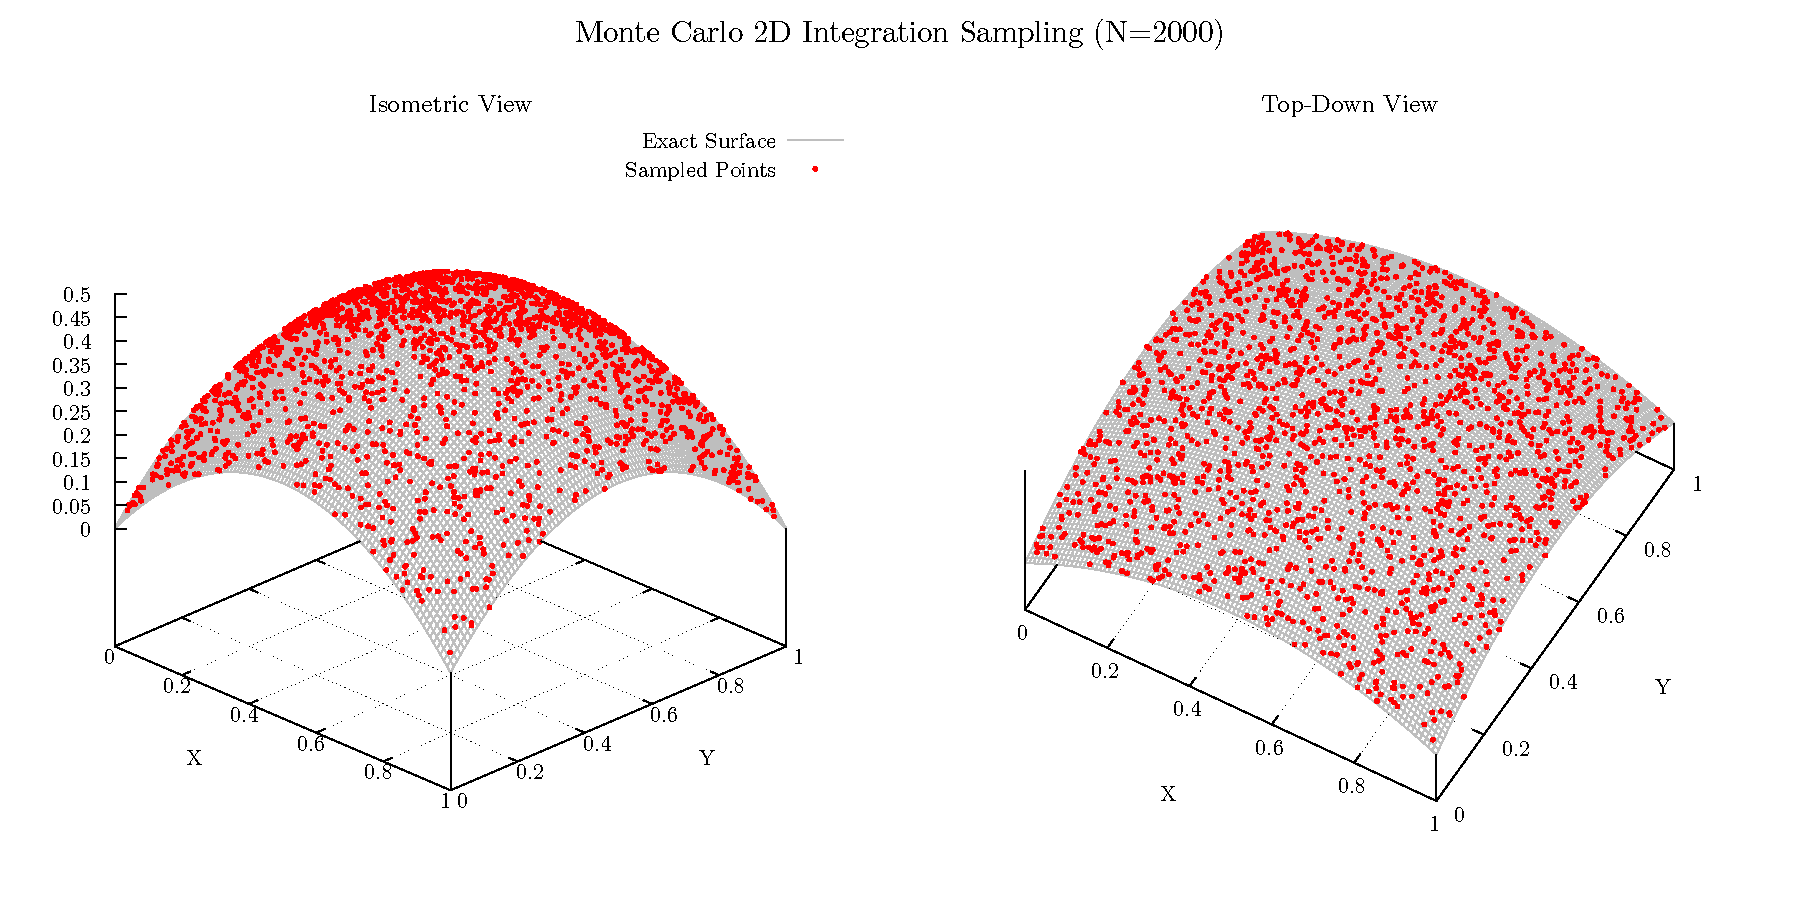
\includegraphics[width=0.8\textwidth]{plots/prob10_multiview.pdf}
                \label{fig16:prob10_sampling}
            \end{figure}
            \item {\bf Output: } \lstinputlisting[style= outputstyle]{output/prob10_output.txt}
        \end{itemize}
        \section{Remarks and Conclusion}
        Based on the computational experiments and subsequent data analysis performed in this study, several key observations regarding Monte Carlo integration methods can be made:
        \begin{enumerate}
            \item {\bf Validation of the Central Limit Theorem:} The empirical results flawlessly reproduced theoretical expectations. Across all tested functions, the log-log curve fitting of the absolute error consistently yielded slopes of approximately $-0.46$ to $-0.50$. This mathematically verifies that the algorithm's statistical error is fundamentally proportional to $\frac{1}{\sqrt{N}}$, confirming the robustness of the pseudorandom number generator used.
            \item {\bf Dimensional Independence and Efficiency:} While deterministic grid-based methods (like the Trapezoidal rule or Simpson's rule) are generally vastly superior for smooth 1D integrals, their computational cost explodes in higher dimensions—a phenomenon known as the "curse of dimensionality." The data in this report proves that the Monte Carlo error convergence rate of $O(N^{-0.5})$ remains completely unaffected when moving from a 1D curve to a 2D surface. This cements Monte Carlo as the most viable numerical method for multi-dimensional thermodynamic and quantum mechanical systems.
            \item {\bf Methodological Trade-offs:} The Hit-or-Miss method proved highly intuitive and exceptionally capable of handling complex, non-linear integration boundaries (such as the circular unit domain). However, it is inherently less efficient than the Mean Value method, as computational resources are "wasted" evaluating and discarding rejected points. The Mean Value method generally produces a lower absolute variance for the same number of samples as it uses every sample point to calculate a weighted average, making it the preferred algorithm when the boundaries are simple.
            \item {\bf The Cost of High Precision:} The $\frac{1}{\sqrt{N}}$ convergence rate, while reliable, is notoriously slow. To achieve just one additional decimal place of accuracy (reducing the error by a factor of 10), the number of computational iterations must increase by a factor of 100. Consequently, while Monte Carlo methods are brilliant for generating rapid approximations of complex multi-dimensional systems, they are highly computationally expensive if strictly high-precision exactness is required.
        \end{enumerate}
        \end{document}